\subsection{Project structure}
In this section we will talk about the structure of the first \acrlong{mvp} of Alastria ID (\textit{\acrshort{mvp}1})\cite{ala-mvp1}.\\
\begin{figure}[h]
    \centering
    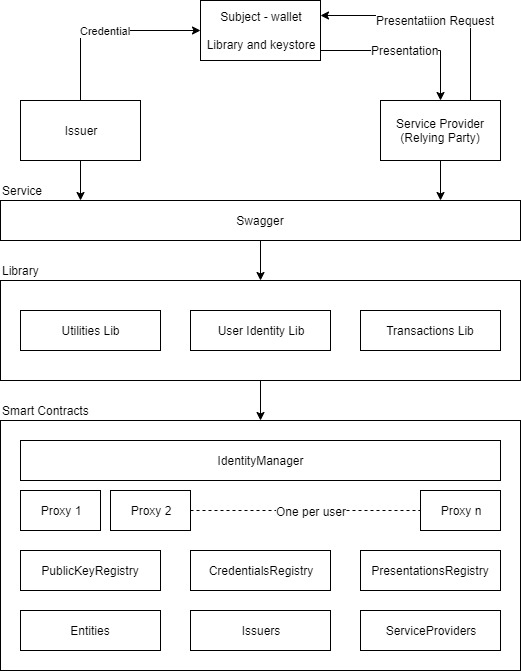
\includegraphics[width=0.7\textwidth]{images/Alastria ID/alastria-mvp1.jpg}
    \caption{Alastria ID MVP1 structure}
    \label{fig:ala_structure}
\end{figure}
The \acrshort{mvp}1 is divided into four main parts, as the figure \ref{fig:ala_structure} shows. Although those are not the only parts that are part of the MVP1. There are another series of components that are very important for the ecosystem, such as:
\begin{itemize}
    \item \textbf{Alastria Node}\footnote{\url{https://github.com/alastria/alastria-node}}: easy documentation and scripts to guide the installation of a blockchain node in the main testnet of Alastria. There are also other guides for different networks, like \textit{Besu}\footnote{\url{https://github.com/alastria/alastria-node-besu}} or \textit{Fabric}\footnote{\url{https://github.com/alastria/alastria-node-fabric}}.
    \item \textbf{Alastria's lib examples}\footnote{\url{https://github.com/alastria/alastria-identity-example}}: use case files to show how to interact with the TypeScript library. This repository is divided according to the different use case that can be done with Alastria ID. There are examples for: creating tokens, creating identities (\acrshort{did}s), creating entities, creating issuers and service providers, creating and deleting credentials and presentations, authentication with Alastria ID, etc.
    \item \textbf{Alastria's objects verification}\footnote{\url{https://github.com/alastria/alastria-identity-JSON-objects}}: this project validates \acrshort{json} objects to see that they are following the specification proposed by Alastria.
\end{itemize}
There are still many repositories to mention, which are somehow auxiliary, or are still work in progress.

\subsubsection{Smart Contracts}
Smart Contracts are the core part of the project, since everything is based on blockchain.\\

It should be mentioned that these Contracts are those created in the first phase of the project (\acrshort{mvp}1). They are not definitive since they have some weaknesses, such as that role governance is not well defined, and they are not Upgradable Smart Contracts.\\

The Smart Contracts are distributed as follows:
\begin{itemize}
    \item \textbf{Identity Smart Contracts}: this set of Smart Contracts are responsible for generating \acrshort{did}s, managing the different roles of the model (Issuers, Service Providers and Subjects) and making calls between the other Contracts to achieve the correct functioning of the implementation.
          \begin{itemize}
              \item \textbf{"AlastriaIdentityManager.sol"}\footnote{\url{https://github.com/alastria/alastria-identity/blob/master/contracts/identityManager/AlastriaIdentityManager.sol}}: this is the main Contract, in charge of creating and managing identities. Contracts \textit{"AlastriaIdentityIssuer.sol"} and \textit{"AlastriaIdentityServiceProvider.sol"} assign roles, and this one creates the identities (\acrshort{did}s). This is the only Contract that is deployed, since it inherits the rest of the "identity" Contracts and is in charge of deploying the "registry" Contracts (figure \ref{fig:mvp1-contracts}).
                    \begin{figure}[h]
                        \centering
                        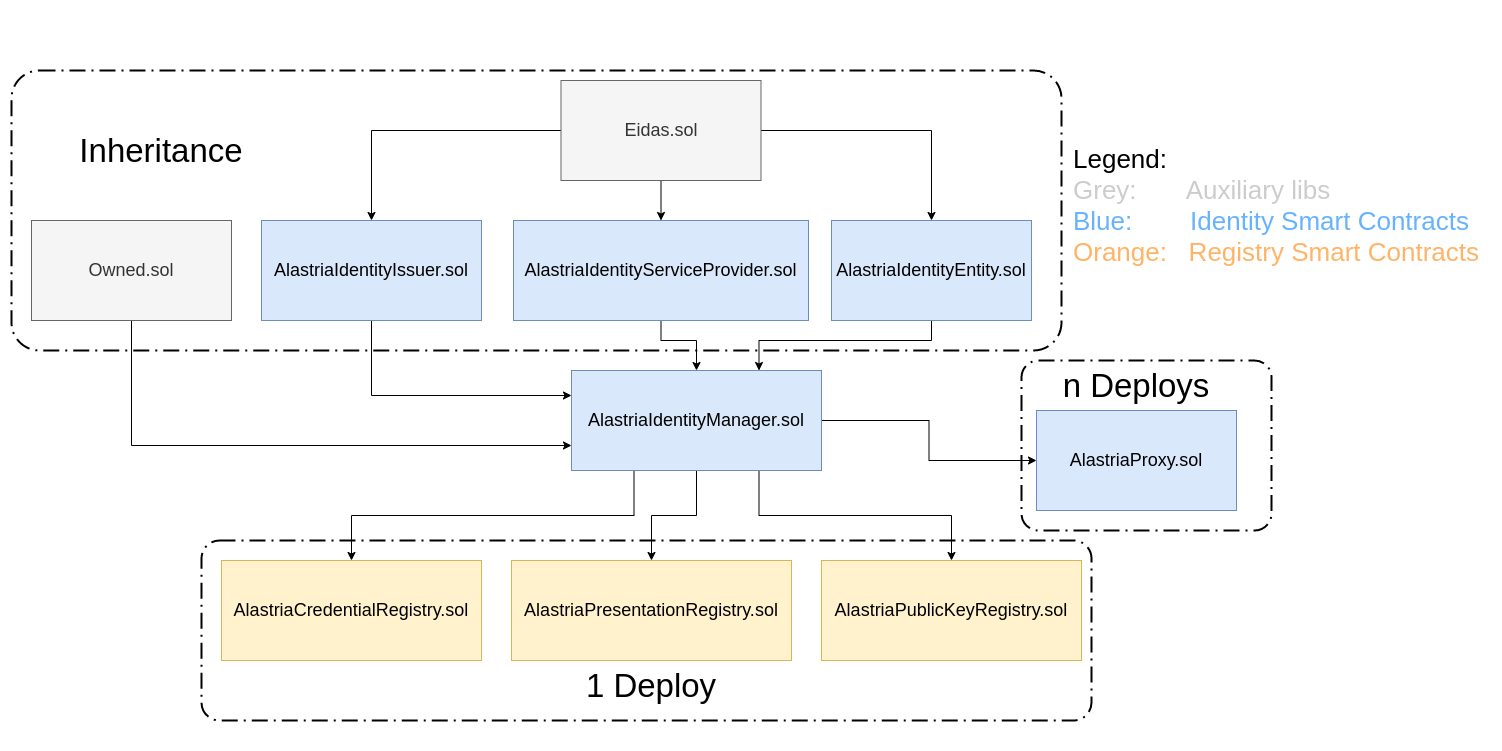
\includegraphics[width=1.1\textwidth]{images/Alastria ID/SCs-Diagram.png}
                        \caption{Alastria ID MVP1 Smart Contracts diagram}
                        \label{fig:mvp1-contracts}
                    \end{figure}
              \item \textbf{"AlastriaIdentityIssuer.sol"}\footnote{\url{https://github.com/alastria/alastria-identity/blob/master/contracts/identityManager/AlastriaIdentityIssuer.sol}}: this Smart Contract is used to endow the entity with the ability to create identities (\acrshort{did}s) and issue Credentials within the blockchain (remember that we are talking about \acrshort{psmh}es, not \acrshort{jwt}s). To do this, the entity is simply saved in a mapping of issuers and the \acrshort{loa} level, using the library \textit{Eidas.sol}.
              \item \textbf{"AlastriaIdentityServiceProvider.sol"}\footnote{\url{https://github.com/alastria/alastria-identity/blob/master/contracts/identityManager/AlastriaIdentityServiceProvider.sol}}: similar to the previous Smart Contract, its functionality is to provide the entities with the role of Service Provider. To do this, it stores the entities in a mapping.
              \item \textbf{"AlastriaIdentityEntity.sol"}\footnote{\url{https://github.com/alastria/alastria-identity/blob/master/contracts/identityManager/AlastriaIdentityEntity.sol}}: it stores entity information, such as name, cif, logo \acrshort{url}, \acrshort{did}, \acrshort{url} of the Alastria Open Access and a flag to know if the entity is active or not.
              \item \textbf{"AlastriaProxy.sol"}\footnote{\url{https://github.com/alastria/alastria-identity/blob/master/contracts/identityManager/AlastriaProxy.sol}}: this Contract, as its name indicates, acts as a proxy for the account \acrshort{eoa} that is carrying out the transaction. Since any call (except for a few) will always go through the account's proxy. It is responsible for emitting an event of what is being used.
          \end{itemize}
    \item \textbf{Registry Smart Contracts}: these are in charge of managing the Credentials and the Presentations with their respective statuses, also it manages the public keys of the different \acrshort{did}s.
          \begin{itemize}
              \item \textbf{"AlastriaCredentialRegistry.sol"}\footnote{\url{https://github.com/alastria/alastria-identity/blob/master/contracts/registry/AlastriaCredentialRegistry.sol}}: it is responsible for managing and modifying the different \acrshort{psmh}es of the Credentials through the different statuses. It should be mentioned that a Credential cannot transits to a "lower" or previous status.
              \item \textbf{"AlastriaPresentationRegistry.sol"}\footnote{\url{https://github.com/alastria/alastria-identity/blob/master/contracts/registry/AlastriaPresentationRegistry.sol}} : this smart contract is analogous to the \textit{"AlastriaCredentialRegistry.sol"} but with the Presentations. Neither the Presentation can transits to a "lower" or previous status.
              \item \textbf{"AlastriaPublicKeyRegistry.sol"}\footnote{\url{https://github.com/alastria/alastria-identity/blob/master/contracts/registry/AlastriaPublicKeyRegistry.sol}}: stores the public keys of the different identities on the network. It has functionalities to add, modify, delete and verify the public keys.
          \end{itemize}
    \item \textbf{Auxiliary libraries}: standard Smart Contracts designed as libraries that are used to facilitate certain actions or improve functionalities of the previous Smart Contracts.
          \begin{itemize}
              \item \textbf{"Eidas.sol"}\footnote{\url{https://github.com/alastria/alastria-identity/blob/master/contracts/libs/Eidas.sol}}: Smart Contract created to comply with the regulations of \acrfull{eidas}.
              \item \textbf{"Owned.sol"}\footnote{\url{https://github.com/alastria/alastria-identity/blob/master/contracts/libs/Owned.sol}}: This is a standard that OpenZeppelin\cite{openzeppelin} has developed that simplifies authorization and control of access to different functions that are implemented in the Smart Contracts.
          \end{itemize}
\end{itemize}

\subsubsection{TypeScript Library}
This library\footnote{\url{https://github.com/alastria/alastria-identity-lib}} written in \textit{TypeScript} has been created to facilitate interaction with Smart Contracts previously mentioned.\\

This library has three different modules:
\begin{itemize}
    \item \textbf{User functions}: it helps to manage the wallet and the identity user. Also helps when signing transactions.
    \item \textbf{Blockchain functions}: it encapsulates the Alastria ID Smart Contracts, so that only functions have to be called with TypeScript, without needing to know how to write in Solidity in order to work with the Smart Contracts. This module is divided as are the Smart Contracts. So, for example, the \textit{"AlastriaPublicKeyRegistry.sol"} can be found in the file \textit{"publicKeyRegistryTransactionFactory.ts"}\footnote{\url{https://github.com/alastria/alastria-identity-lib/blob/master/src/txFactory/publicKeyRegistryTransactionFactory.ts}}. It is the same for the rest of the main Smart Contracts.
    \item \textbf{Tokens functions}: it manages the different \acrshort{jwt}s explained previously, guaranteeing that they are well built and are valid. It also allows the signing and decoding of said \acrshort{jwt}s.
\end{itemize}

\subsubsection{Wallet}
The Alastria ID wallet\footnote{\url{https://github.com/alastria/alastria-wallet}}, is a mobile application written in \textit{Ionic} to implement the different user stories of Alastria ID. This wallet is a \acrfull{poc}, which means it is not a valid wallet for a project in production. This is because it does many things in a "fake way" since the objective was not to be a commercial product.\\

In the secure part of the wallet (called \textit{secure storage}) the keys are generated and stored that users use to sign and verify such signatures. Herein lies one of the main problems of this wallet, since it is not a \textit{multidivice wallet}, that is, each pair of keys is only and only for one device (wallet). Another of the main problems is that the key recovery or modification flow has not yet been defined, so if the wallet is removed from the device, the identity would be lost.\\

To finish this section, we will explain what and how are the keys that are stored in the wallet are. This keys are called \textit{keystores}. This \textit{keystores} is nothing other than an \acrfull{eoa} used to interact with the blockchain. The listing \ref{lst:keystore} shows an example of a \textit{keystore}.
\lstinputlisting[language=json,label={lst:keystore}, caption=Keystore example]{examples/codeSnippets/keystore.json}

\subsubsection{Entity}
It is called "Entity" to an example implementation to simulate an entity\footnote{\url{https://github.com/alastria/alastria-identity-entity}}. This entity has both roles, Issuer and Service Provider. It is designed to interact with the wallet to perform the full \acrshort{poc} for the \acrshort{mvp}1. It contains a \textit{Mongo} database that is used to store certain information.\\

This implementation is divided into two parts: the backend and the frontend.
\begin{itemize}
    \item \textbf{Backend}: written with \textit{Swagger} and \textit{NodeJS} and it is in charge of interacting with the Smart Contracts, making use of the previously mentioned \textit{TypeScript} library. The following operations can be performed: create an identity (\acrshort{did}), issue Credentials and receive Presentations, as well as check the statuses of both. It stores and reads information in the database.
    \item \textbf{Frontend}: developed with \textit{Angular}, \textit{JavaScript} and \textit{Nginx}. It is the facade to interact with the backend and offer a better user experience than by using scripts. Currently it can be checked online\footnote{As it is a temporary demo, it may no longer be operational \url{http://34.244.47.233/login}}.
\end{itemize}